\chapter{Reproduktion bisheriger Ergebnisse}
\label{chap:reproduktion}
\epigraph{What I cannot create, I do not understand}{--- Richard Feyman}

\qq{Warum NN?}
Künstliche Neuronale Netzwerke (kurz NN) dominieren den Forschungsbereich der 
Bilderkennung. 
Besonders die Klasse der faltenden Neuronalen Netzwerks \engl{convolutional neural network}, kurz CNN, konnte viele Erfolge für sich beanspruchen.
Rekordbrechende Ergebnisse bei der Klassifiziererung von handgeschriebenen Ziffern \parencite{LeCunBackpropagationappliedhandwritten1989} und des ImageNet-Wettbewerbs \parencite{KrizhevskyImageNetClassificationDeep2012a} motivieren dazu CNN-Methoden auch in anderen
Bereichen anzuwenden.

\begin{marginfigure}
    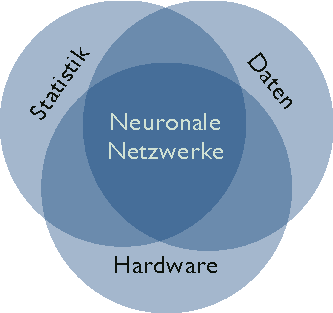
\includegraphics[width=\textwidth]{figures/tasks/nn_areas_venn.pdf}
    \caption{Diziplinen im Bereich Neurale Netzwerke}
    \label{fig:chen:cnn_task}
\end{marginfigure}
Neurale Netzwerke benötigen weniger Entwicklungsaufwand und können zudem einfacher von 
 wachsenden Rechenkapazitäten und Datenmengen gebrauch machen \parencite[436]{LeCunDeeplearning2015}. 
Aber die Wissenschaft der NN ist ein Feld, dass durch die aktuelle Praxis mehr als durch Theorie geprägt ist. 
Das bedeuted zum einen das theoretische Grundlagen noch nicht gefestigt sind.
Zum anderen ist die Theorie nur eine Faktor für den erfolgreichen Einsatz von NNs. 
Je mehr Parameter unklar sind desto schwieriger wird eine Reproduktion.
\qq{Unterschied replikation, reproduktion?}
Die Reproduktion von Ergebnissen ist aber ein wichtiger Bestandteil in jedem Forschungsgebiet. 

\qq{welche Experimente?}
Im folgenden werden Paper genauer untersucht, die sich mit dem Problem der Dokumentensegmentierung mit Hilfe von CNNs nähern.
Das erste Experiment basiert auf dem neusten Paper von Mitgliedern der DIVA-Gruppe: \citeauthor*{ChenConvolutionalNeuralNetworks2017}. 

Das zweite Experiment basiert auf der Forschung des Gewinners des IDCAR2017-Wettbewerbs: \citeauthor*{XuPageSegmentationHistorical2017} 

\section{Andere Ansätze}
\cite{WickFullyConvolutionalNeural2017}


\section{Einführung Maschinelles Lernen}
Neurale Netwerke und CNN sind Beispiele für Machinenlernalgorithmen \engl{maschine learning algorithms}.
\cite{MitchellMachinelearning1997} definiert einen Machinenlernalgorithmus wie folgt: ``A computer program is said to learn from experience E with respect to some class of tasks T and perfomance measure P, if its performance at tasks T, as measured by P improves with experience E''.

% experience E 
Die Erfahrung E kann zum Beispiel ein Datensatz \(X\) mit zugehörigen Klassen
\(Y\) sein. Im Fall der Dokumentensegmentierung kann ein Element \(x_i\) ein Bildauschnitt sein, 
dessen Kategorisierung ist dann das Label \(y_i\)(siehe \cref{fig:chen:cnn_task}).
\begin{marginfigure}
    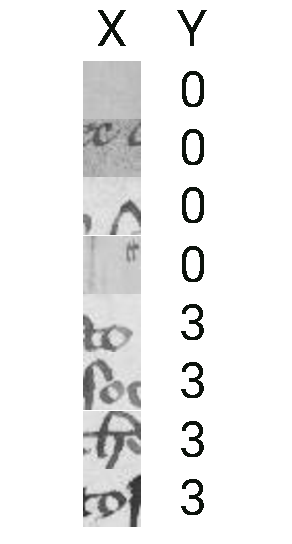
\includegraphics[width=\textwidth]{figures/tasks/chen_examples.pdf}
    \caption{Bildauschnitt mit ground ground truh (0: Hintergrund, 3: Haupttext)}
    \label{fig:chen:cnn_task}
\end{marginfigure}

% Task T 
Die Aufgabe T ist für die meisten Anwendungen eine Klassifizierungsaufgabe. 
Der Lernalgorithmus soll dabei eine Funktion finden \(f: \mathds{R}^n \rightarrow \left\{1,\dots,k \right\} \) so das \(y = f\left(x\right)\) \parencite[97 ff]{GoodfellowDeeplearning2016}.
Ein Lernalgorithmus der diese Funktion findet ist ein überwachter Lernalgorithmus \engl{supervised learning algorithm}
Der Algorithmus versucht die Wahrscheinlichkeitsverteilung \(p(y | x)\) implizit zu ``lernen''. Ein unüberwachter Lernalgorithmus versucht die Verteilung \(p(x)\) direkt zu lernen.
Die Trennung zwischen überwacht und unüberwacht ist nur eine grobe Einteilung. Tätsächlich sind die übergänge fließend. 
Manche Machinenlernverfahren benutzen beide Methoden.  

% perfrmance P
Die Performanz P der Vorhersagefunktion \(f\) wird im einfachsten Fall mit der Genauigkeit,
dem Verhähltniss von richtigen Vorhersage zu Falschen, gemessen. 
% TODO: Tabelle
\cref{tab:truth}
\begin{table}
    \caption{Wahrheitstabelle}
    \label{tab:truth}
    \begin{tabular}{llll}
                    &&\(y\)& \\
                            && Positiv       & Negativ \\
    \(\hat{y}\) & Positiv  & true positive  & false positive \\
                & Negativ & false negatve   & true negatve \\
    \end{tabular}       
\end{table}    
\section{Künstliche Neuronale Netzwerke}

Künstliche Neurale Netwerke sind eine Methode des statistischen Lernens die von der Natur inspiriert wurde. 
Das Neuron ist der Grundbaustein eines Netwerkes und verarbeitet eingehende Signale. 
Nur ein Signal wird

\begin{align}
    \hat { y } = w^{ \top } x + b
\end{align}

\begin{align}
    f(X)=\sum\limits_{m=1}^{M}g_{m}\left(\omega_{m}^{\top}X\right)
   \end{align}
Target als nonlineare Funktion dieser Features modelieren.  


\section{SGD}

\section{Aktivierungsfunktionen}
\begin{align}
    \operatorname{softmax}(z)_{i}=\frac{\exp\left(z_{i}\right)}{ \sum _ { j } \exp \left( z _ { j } \right) }
\end{align}
% TODO: set font size??? 
\begin{figure}
    \caption{ReLU- und Sigmoid-Funktionsplot}
    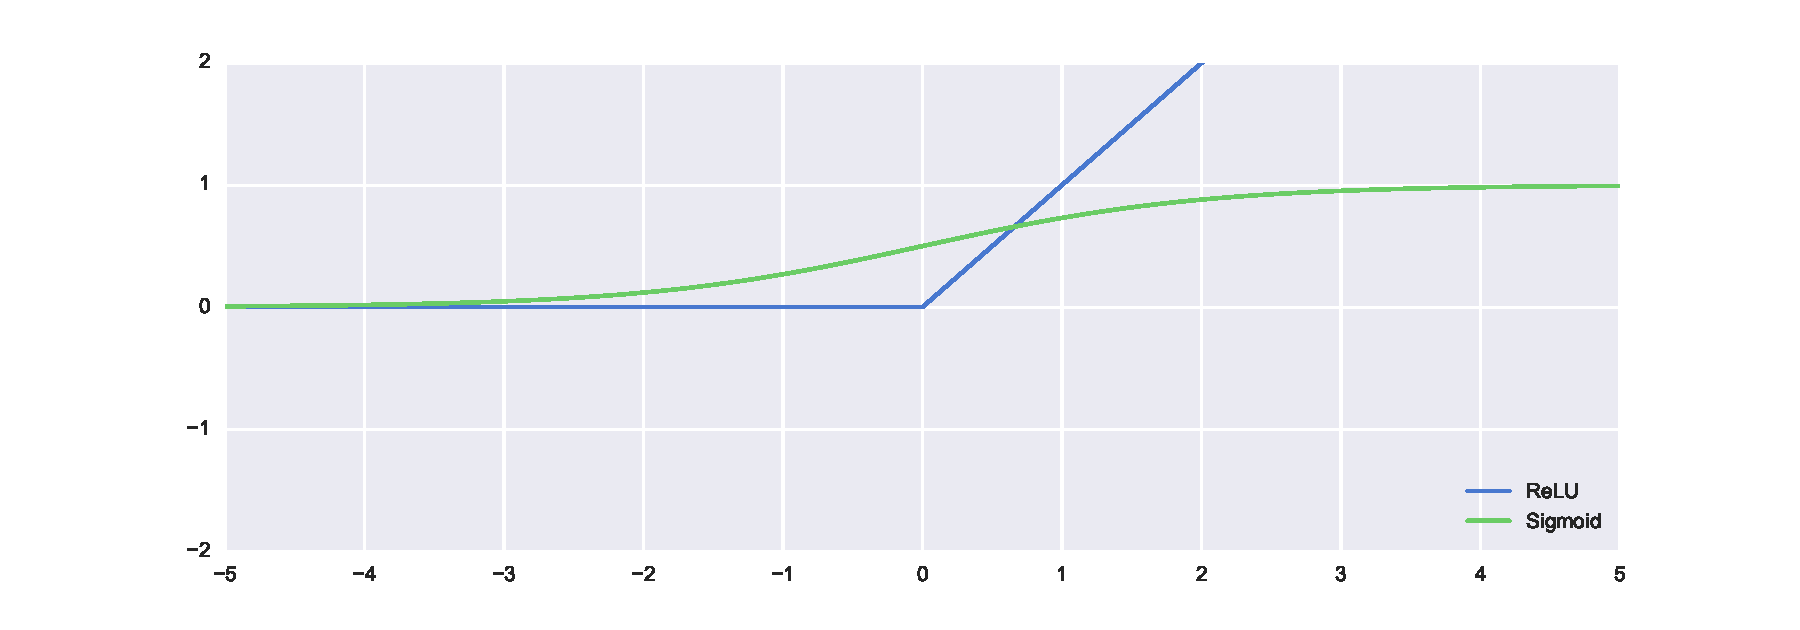
\includegraphics[width=\textwidth]{figures/plot/relu_sigmoid.pdf}
\end{figure}

\subsection{ReLU}
\begin{align}
    f\left(x\right) &= \text{max}(0,x)
\end{align}
\subsection{Softmax}

\subsection{Regularisierung}
\label{sec:Regularisierung}

\section{CNN}
\qq{Nachtteile fully connected NN für Bilderverarbeitung}
Die Anzahl der Parameter in der Gewichtsmatrix \(W\) wird von der Größe des Inputs bestimmt.
Möchte man Bilder ein Bild mit der der 

\qq{Sind Filter vorläufer von CNN?}
CNN kombinieren zwei Konzepte der Bilderverarbeitung: Neuronale Netzwerke und Filter.
Klassifikationsprobleme wurde traditionell in zwei Schritten gelöst. Zuerst wurden 
Featuredeskriptoren entwickelt welche dann als Input für trainierbare Klassifizierer 
verwendet wurden \autocite[2353]{RawatDeepConvolutionalNeural2017}.


\qq{Was ist convolutional?}
So können zum Beipspiel Kanten in einem Bild ein Klassifizerungsgrundbaustein sein. 
Um die Kanten in einem Bild zu finden wird das Bild mit einem Kernel  gefaltet.  
Der Begriff Faltung wird üblicherweise für die Verknüpfung von zwei realwertigen Funktione verwendet. Die analoge Form der Faltung ist eine lineare , translations-invariante Funktion, siehe \cite[28]{SusseBildverarbeitungundObjekterkennung2014}. 
\begin{align}
    \label{eq:convolutional}
    convolutional
\end{align}
Im Bereich der Bilderverarbeitung wird schon länger eine abgeänderte Faltungsfunktion genutzt: die Autokorrelation \engl{cross-correlation}. Bild und Filter sind 2D-Funktionen die zum einen nur für diskrete Intervale definiert sind zum anderen für Bereiche aushalb des ihres Definitionsbereichs gleich 0 sind. Zudem wird überlicherweise der Index für den Kernel addiert (siehe \cref{eq:convolutional}).
\begin{align}
    \label{eq:crosscorrelation}
    I*K(i,j) =
\end{align}


Ein CNN ist eine Neurales Netzwerk, dass in mindesten einen Layer die Faltung anstatt der normalen Matrixmultiplikation verwendet \parencite[321]{GoodfellowDeeplearning2016}.
\qq{Drei Hauptvorteile?}
\cite{GoodfellowDeeplearning2016} sieht drei Vorteile von CNN gegenüber voll-vernetzten NN: verringerte Konnektivität, 
gemeinsame Parameternutzung, eqivariante Darstellung.
Wie schon erwahnt steigt die Anzahl der Parameter in einem voll-vernetzten NN je größer der Input wird, weil jedes Neuron mit jeder Aktivierung der vorhergehenden Schicht verbunden ist. 
Durch die Faltungssoperation erhählt jedes Neuron nur die Signale die im Bereich des Filterkernels liegen. Dieser Bereich wird auch rezeptives Feld genannnt.
Durch die Schichtung von mehreren Faltungen vergrößert sich das rezeptive Feld der Neuronen in tieferen Schichten (siehe \cref{fig:cnn_neurons}).


\begin{marginfigure}
    \label{fig:cnn_neurons}
    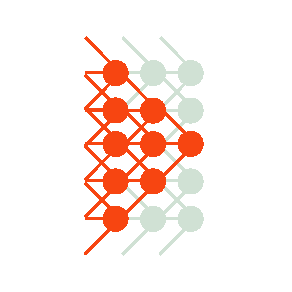
\includegraphics[width=\textwidth]{figures/sketch/cnn/perceptive_field.pdf}
    \caption{Rezeptives Feld in einem mehrschichtigen Netz}
\end{marginfigure}

\qq{Nachteile CNN?}
\qq{Filterbeispiel?}
\qq{}

\section{\textcite{ChenConvolutionalNeuralNetworks2017}}
Das Paper ``\citetitle*{ChenConvolutionalNeuralNetworks2017}'' von \citeauthor*{ChenConvolutionalNeuralNetworks2017} betrachten die Dokumentensegmentierung 
als ``pixel labeling problem''. Einem Pixel wird eine Klasse zugewiesen indem
ein CNN die Umgebung des Pixels analisiert. 
Jedoch ist eines der größten Probleme bei der Verarbeitung von Dokumentenseiten die Größe.
Die Bilder im HisDB-Datenset sind mit einer Auflösung von \(4872 \times 6496\) wesentlich größer als andere Datensets.\qq{Welche?}
Um den Prozess zu beschleunigen werden nicht alle Pixel sondern nur etwa 3000 Pixelcluster klassifiziert. 

\subsection{Vorverarbeitung}
\citeauthor{ChenConvolutionalNeuralNetworks2017} skalieren alle Bilder mit einem Faktor von  \(2^{-3}\) und wenden dann den Superpixelalgorithmus SLIC (simple linerar iterative clustering) an \parencite{AchantaSLICSuperpixels2010} um die Dokumentenseiten in Superpixel einzuteilen.
Ein \(28 \times 28\)-Bereich um das Zentrum des Superpixel wird dann mithilfe eines CNN
klassifiziert. Diese Klassifizierung wird dann allen Pixel innerhalb des Superpixels zugewiesen.

\section{SLIC Superpixel}
Der SLIC-Algorithmus basiert auf dem k-Means-Algorithmus und teilt Pixel inhalb eines 5D-Raums in Cluster ein. 
In jedem Arbeitsschritt werden Pixel dem Clusterzentrum mit der geringsten Distanz zugeordnet und danach werden die Clusterzentren neu berechnet.
Das Distanzmaß \(D_s\) zu den Clusterzentren \(k=[1,K]\) basiert auf den Farbabstand im Lab-Farbraum \(d_{lab}\) und den räumlichen Abstand \(d_{xy}\):

\begin{align}
    d_{lab} &= \sqrt{ \left( l_k - l_i \right)^2 + \left( a_k - a_i \right)^2 + \left( b_k - b_i \right)^2 }\\
    d_{xy}  &= \sqrt{ \left( x_k - x_i \right)^2 + \left(y_k - y_i \right)^2 }\\
    D_{s}   &= d_{lab} + \frac{m}{S} d_{xy}
\end{align}

Der Faktor \(m\) ermöglicht eine Gewichtung den zwei Distanzmaßen. Je höher
der Faktor desto kompakter werden die Superpixel. \cref{fig:slic_parameters}
zeigt das Ergebniss des Algorithmus mit unterschiedlichen Parameter  \(m\)
angewendet auf eine Dokumentenseite.

\begin{figure}
    \centering
    \caption{Die SLIC-Pixelgrenzen sind in rot dargestellt }
    \label{fig:slic_parameters}
    \subfloat[ \(m = 0.1\)]{
        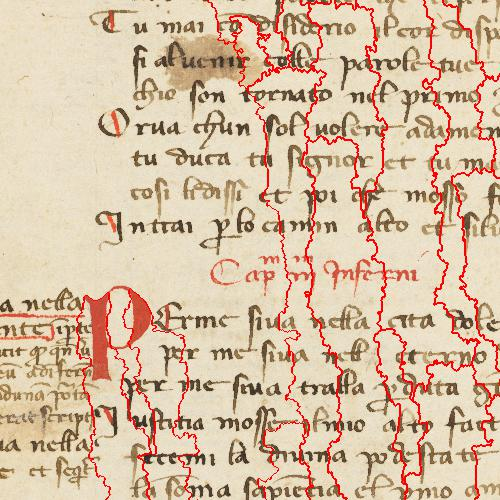
\includegraphics[width=0.24\textwidth]{figures/img/mark_boundaries_m0.jpg}
    }
    \subfloat[\(m = 1\)]{
        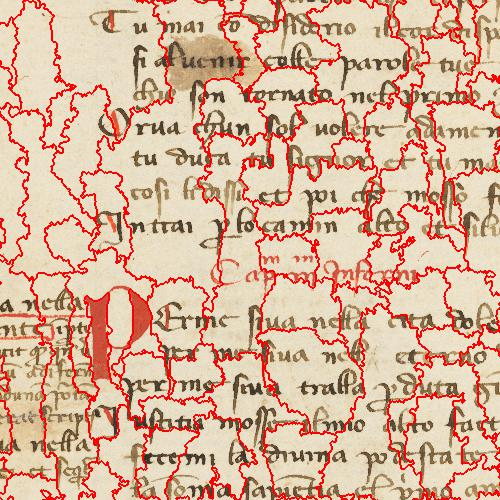
\includegraphics[width=0.24\textwidth]{figures/img/mark_boundaries_m1.jpg}
    }
    \subfloat[\(m = 10\)]{
        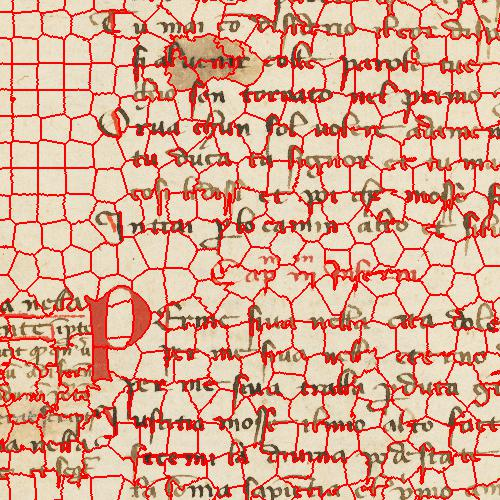
\includegraphics[width=0.24\textwidth]{figures/img/mark_boundaries_m10.jpg}
    }
    \subfloat[\(m = 100\)]{
        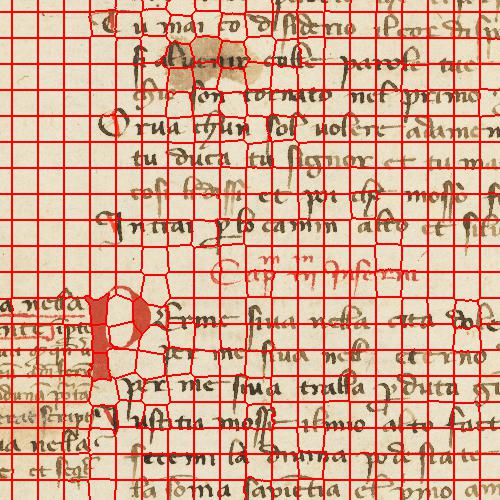
\includegraphics[width=0.24\textwidth]{figures/img/mark_boundaries_m100.jpg}
    }
\end{figure}

\citeauthor{AchantaSLICSuperpixelsCompared2012} stellen später zwei wichtige Erweiterungen vor:
Normalisierung des Distanzmaßes und Adaptive-SLIC.

\citeauthor{ChenConvolutionalNeuralNetworks2017a} nennen keine Details zur Wahl
der Superpixel-Parameter, nennen aber eine frühere Studie die sich mit unterschiedlichen 
Superpixel verfahren beschäftigt \parencite{ChenPageSegmentationHistorical2016}.
Die Studie versucht einen Autoencoder (siehe \ref{sec:autoencoder}) zu trainieren auf Basis von Superpixeln und vergleicht dabei den Einfluss von unterschiedlichen Superpixel-Methoden. Die veröffenlichen Ergebniss zeigen aber nur die Performanz im Bezug
auf die Zahl der Cluster \(n \in \left\{10^3, 50^3, 100^3, 200^3\right\}\) und dem Skalierungsfaktor \(\alpha \in \left\{2^{-2}, 2^{-3}\right\}\)
\qq{adaptive slic}
\qq{Problem gt zu treffen}

\section{CNN-Architektur}
\citeauthor{ChenConvolutionalNeuralNetworks2017a} beschreiben die Struktur
des CNN als \(28 \times 28 \times 1 - 26 \times 26 \times 4 - 100 - M\).

Während des Trainings wird das Ground-truth Label des Zentrumpixels als Label für den Superpixel verwendet.


\section{Xavier initialization}


\section{Dropout}



\section{Training}


\section{\textcite{XuPageSegmentationHistorical2017}}
Das Paper \citetitle*{XuPageSegmentationHistorical2017} von \citeauthor*{XuPageSegmentationHistorical2017} verfolgt einen anderen Ansatz.
\citeauthor{XuPageSegmentationHistorical2017} verwenden eine Netwerk  


\section{VGG}
\section{Deconvolution}
\section{Ergebnisse}